% !TEX root = ../main.tex

% 中英标题：\chapter{中文标题}[英文标题]
\chapter{噪声感知与偏好提取的多模态多行为推荐方法}

\section{引言}

随着推荐系统在电商、短视频与内容分发等场景中的广泛应用，用户行为数据呈现出多样化和复杂化的特征。不同类型的用户行为（如点击、收藏、购买等）蕴含了用户多层次的兴趣线索，为建模个性化偏好提供了丰富的信息来源。然而，当前推荐系统在建模用户偏好时仍面临两大核心挑战：其一，多行为交互数据中普遍存在噪声，例如误点击、无效浏览等行为可能不能准确反映用户的真实兴趣；其二，现有方法主要依赖用户–物品的协同信号，忽视了物品本身的多模态语义内容（如文本描述和图像特征），从而限制了模型在兴趣表达不充分或行为多样性较高场景下的建模能力。

近年来，针对多行为推荐问题的研究逐渐深入，已有工作主要集中在行为关系建模和行为融合策略上，通过在不同层次捕获多行为间的关联性来提升推荐效果。然而，这些方法普遍存在两方面不足：一方面，它们通常假设辅助行为均为有效信号，未能充分考虑行为数据中的噪声问题，导致模型可能受到误导性交互干扰；另一方面，尽管多模态信息（如图像和文本）能够为用户偏好提供语义补充，但现有研究往往将其作为静态特征使用，缺乏与多行为信号的深度融合，难以实现语义层面的偏好理解与去噪。

针对上述问题，本章主要研究以下关键问题：如何在多行为推荐系统中识别并抑制噪声交互？如何将多模态内容特征与多行为信号进行有效融合，从而提升用户偏好表示的准确性与稳健性？本章提出的方法将多模态信息（文本、图像）与多行为交互信号协同建模，并通过图神经网络和对比学习机制实现语义增强和噪声抑制，为解决上述问题提供技术方案。

\section{问题定义及方法概述}
\subsection{问题定义}
在本研究中，设用户集合为 $\mathcal{U}=\{u_1, u_2, \ldots, u_{|\mathcal{U}|}\}$，物品集合为 $\mathcal{I}=\{i_1, i_2, \ldots, i_{|\mathcal{I}|}\}$。定义用户–物品交互图为
\begin{equation}
    G^R = (V, E^R),
\end{equation}
其中，节点集合 $V = \mathcal{U} \cup \mathcal{I}$ 表示所有用户与物品节点，边集合 $E^R$ 表示观测到的用户–物品交互关系。在多行为场景下，用户可能与同一物品发生多种类型的交互（如浏览、加购、购买等）。因此，整体交互图 $G^R$ 可以划分为 $K$ 个行为子图：
\begin{equation}
    G^R = \{G^R_1, G^R_2, \ldots, G^R_K\},
\end{equation}
其中，$G^R_k$ 表示第 $k$ 种行为对应的子图。

为便于建模，定义交互矩阵集合 $\{R_1, R_2, \ldots, R_K\}$，其中
\begin{equation}
    R_k \in \mathbb{R}^{|\mathcal{U}| \times |\mathcal{I}|}
\end{equation}
表示行为 $k$ 下的用户–物品交互矩阵。若
\begin{equation}
    R^k_{ui} = 1,
\end{equation}
则表示用户 $u$ 在行为 $k$ 下与物品 $i$ 发生过交互，对应地，在行为图 $G^R_k$ 中存在一条连接用户 $u$ 与物品 $i$ 的边；若
\begin{equation}
    R^k_{ui} = 0,
\end{equation}
则表示该交互未发生。

在推荐任务中，模型旨在学习一个预测函数 $\widehat{y}_{ui}$，用于刻画用户 $u$ 对物品 $i$ 的偏好强度：
\begin{equation}
    \widehat{y}_{ui} = f(u, i \, | \, \Theta),
\end{equation}
其中 $f(\cdot)$ 表示推荐模型，$\Theta$ 为模型参数。根据预测得分对物品集合 $\mathcal{I}$ 进行排序，可为用户 $u$ 生成推荐列表 $R_u$，即排名最高的 Top-$K$ 个物品：
\begin{equation}
    R_u = \text{Top-}K(\widehat{y}_{ui}, \, i \in \mathcal{I}).
\end{equation}

综上，多行为推荐任务的形式化定义如下：
\begin{itemize}
    \item \textbf{输入：} 用户在 $K$ 种行为下的交互图集合 $\{G^R_1, G^R_2, \ldots, G^R_K\}$；
    \item \textbf{输出：} 一个推荐模型，用于预测用户 $u$ 在第 $K$ 种行为（即目标行为）下与物品 $i$ 发生交互的概率 $\widehat{y}_{ui}$。
\end{itemize}

\subsection{算法概述}

\begin{figure}[h]
\centering
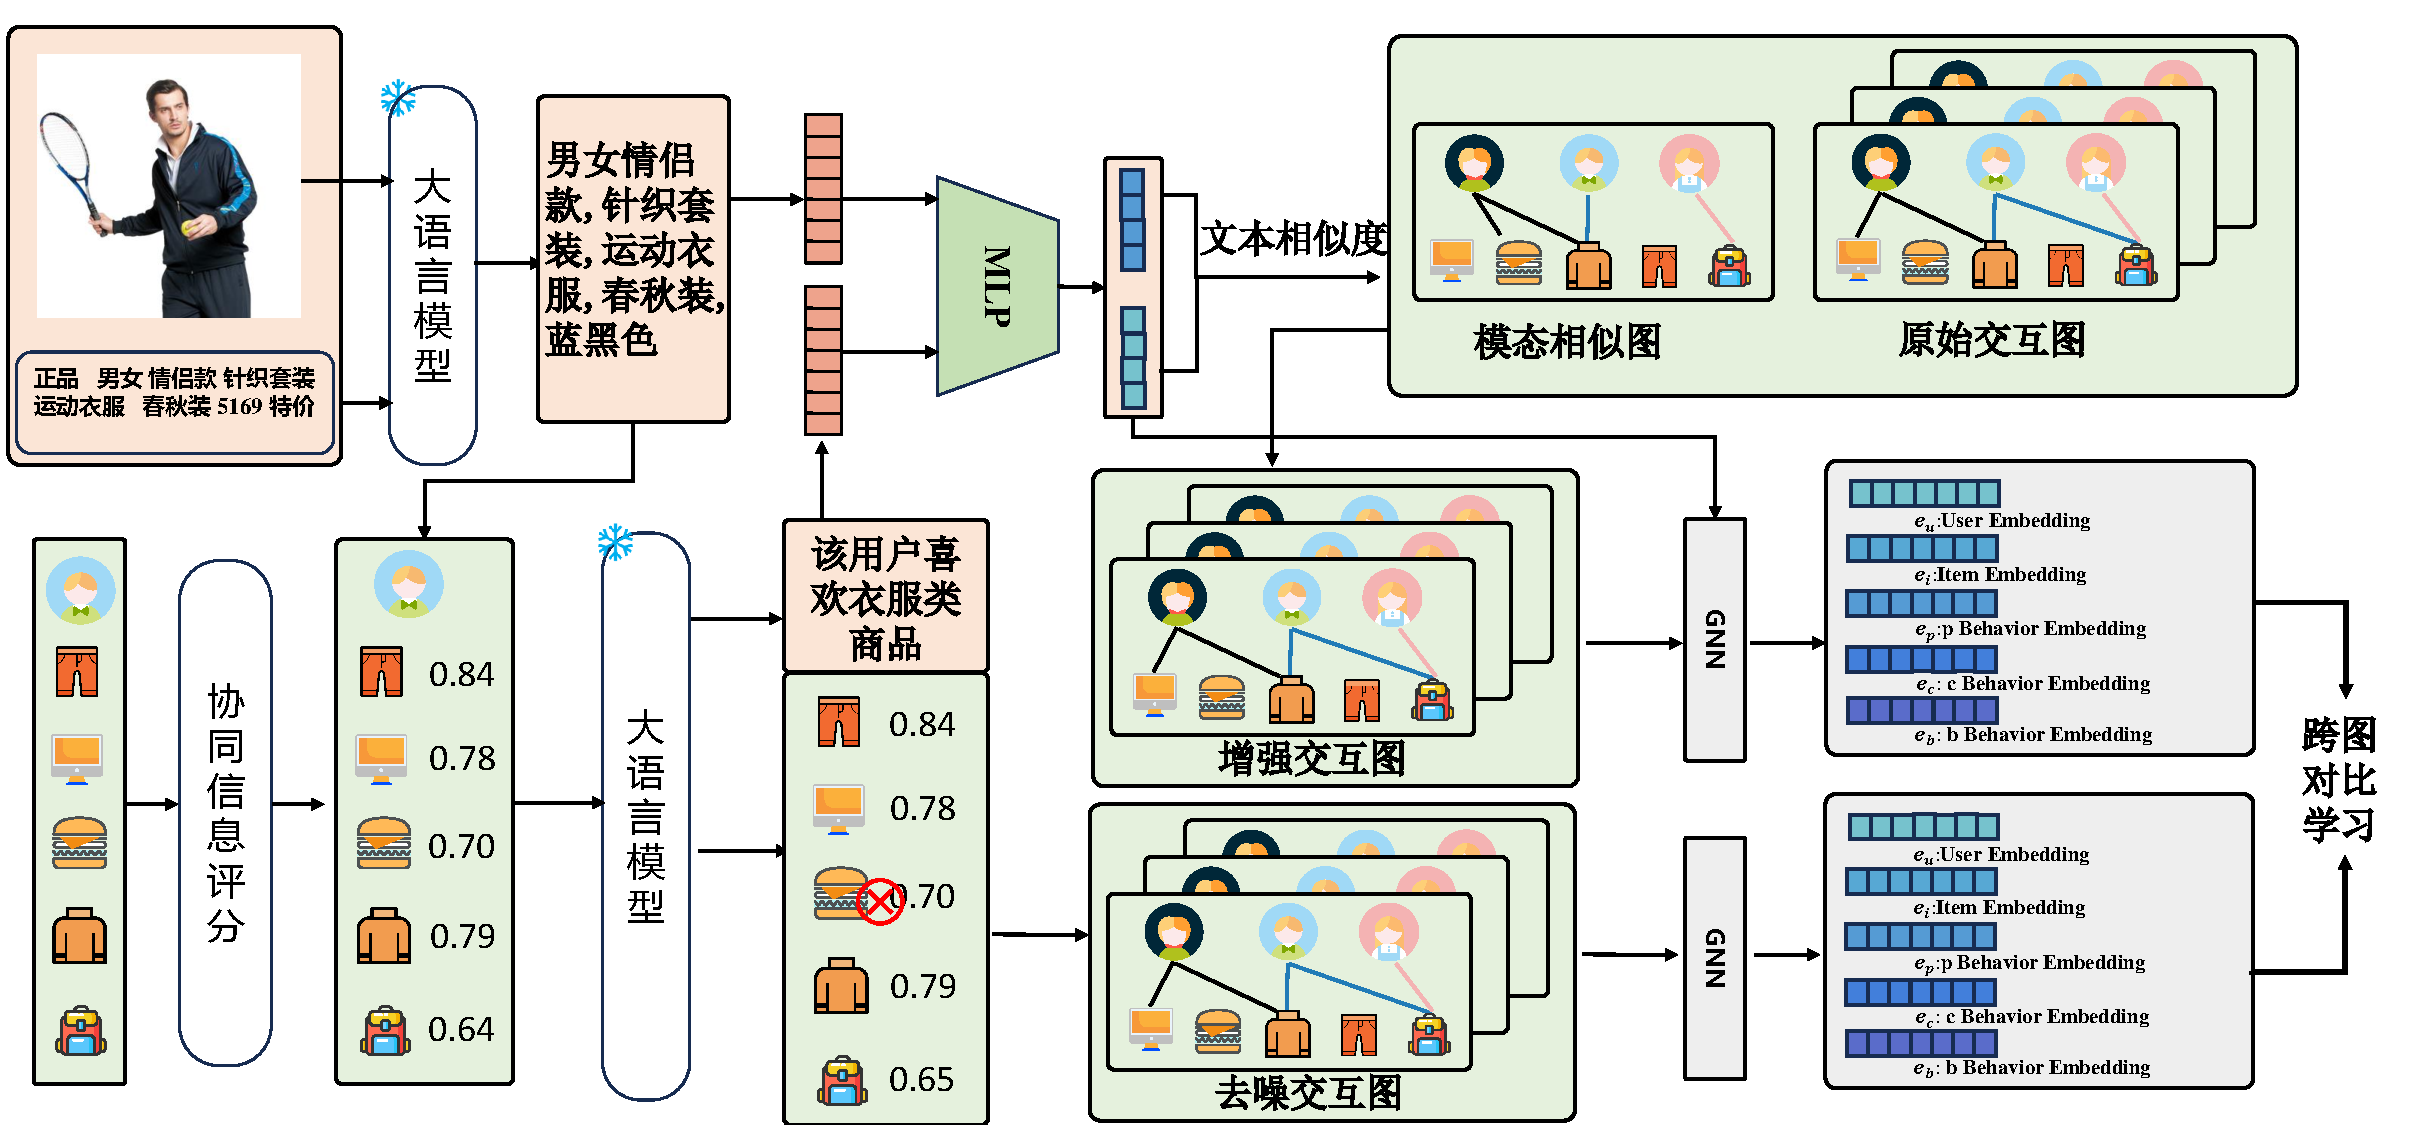
\includegraphics[width = 1.0\textwidth]{figures/model2.pdf}
\caption{噪声感知与偏好提取的多模态多行为推荐方法整体框架示意图}
\label{fig:model2}
\end{figure}

本研究聚焦于多模态多行为推荐系统中的噪声干扰与鲁棒表示建模问题，提出了一种统一的多模态多行为去噪推荐框架。该方法融合了大语言模型的语义生成能力、多模态内容理解、图神经网络的结构建模优势以及对比学习的判别特性，以实现高质量、可解释且鲁棒的用户–物品表示学习。整体框架由以下三个核心模块组成：

\textbf{多模态辅助偏好建模模块。}
为获得语义丰富且具备判别力的特征表示，本文首先利用 LLM 对多模态内容进行语义对齐。具体而言，物品侧基于图像与文本模态信息，通过 LLM 生成内容一致的语义文本描述，并将不同模态特征映射至共享语义空间，实现模态间的对齐与融合。随后，利用生成的模态嵌入计算用户–物品交互的语义相似度，并根据相似度阈值执行\textbf{硬去噪}，以剔除显著偏离用户真实兴趣的异常交互行为。针对多模态推荐中的文本特征提取问题，现有方法通常直接使用原始文本或独立编码各模态特征，存在不同模态间语义偏差较大的问题。本文提出的方法的特殊之处在于：在文本提取之前，首先利用大语言模型引入其世界知识，将原始文本与图像信息进行融合，生成语义一致的文本描述。通过这一预处理步骤，不同模态的信息被统一映射到共享语义空间，从而显著减少了多模态推荐中常见的模态间语义偏差问题。相较于传统方法，本方法能够更准确地捕获用户偏好与物品语义之间的真实关联，提高下游推荐任务的效果与鲁棒性。

\textbf{语义感知的图消息传递模块。}
为联合建模交互结构与模态语义信息，本文设计了一种语义感知的消息传递机制。在邻居聚合过程中，引入基于模态相似度的注意力加权策略，使图神经网络在传播阶段重点聚合语义一致性更高的邻居节点；在特征更新阶段，融合交互嵌入、行为类型嵌入与模态语义嵌入，从而捕获多源特征间的互补关系，提升用户与物品表示的表达能力。

\textbf{模态感知图增强与对比学习模块。}
为弥补原始交互图中潜在的偏好缺失，本文基于多模态语义关系构建语义增强图 $\mathcal{G}_{\text{aug}}$，并将其与去噪后的协同交互图共同用于表示学习。通过引入图级对比学习策略，对两种视角下的节点表示进行对齐，使模型能够在结构空间与语义空间之间实现一致性约束与知识迁移，从而有效提升推荐的鲁棒性与泛化性能。

\subsubsection{复杂度分析}
本章所提出的多模态多行为去噪推荐方法主要包含三个核心模块：多模态辅助偏好建模模块、语义感知的图消息传递模块以及模态感知图增强与对比学习模块。  

在多模态辅助偏好建模阶段，利用LLM生成物品模态嵌入并进行语义对齐，其时间复杂度取决于文本/图像长度 $L$ 与嵌入维度 $d_m$，可表示为 $O(L \cdot d_m^2)$。硬去噪操作基于用户-物品相似度筛选异常交互，复杂度为 $O(|E|)$。  

在语义感知的图消息传递阶段，引入模态注意力加权的邻居聚合操作，其复杂度为 $O(|U| \cdot k \cdot d_\text{total})$，其中 $d_\text{total}$ 为融合后的总嵌入维度。  

在模态感知图增强与对比学习阶段，对节点进行图级对比学习，其复杂度为 $O(|U| \cdot S \cdot d_\text{total})$，$S$ 为每个用户采样的正负样本数。空间复杂度主要包括用户与物品嵌入、正负样本缓存及模态嵌入，总体为 $O((|U|+|I|) \cdot (d+d_m) + |U| \cdot S + |E|)$。整体设计保证方法在处理大规模多行为与多模态交互数据时仍具有良好的可扩展性。

\section{多模态辅助偏好建模}
\textbf{多模态输入与文本摘要生成：}  
本研究的输入数据包括物品侧的图像与标题文本，以及用户侧的多行为交互记录。物品侧数据通常存在语义噪声：图像中可能包含广告、水印或背景干扰元素，而文本标题多由商家编写，常含有营销性修辞或冗余关键词，难以准确反映商品的核心属性。为实现多模态内容的统一理解与语义浓缩表达，物品的图像与文本标题被共同输入至多模态大语言模型（LLM），通过设计提示词（prompt），在视觉与文本的协同语义空间中生成高质量的物品摘要文本。

如图\ref{fig:prompt1}所示，在提示设计中，输入由“任务指令部分”和“数据输入部分”组成。  
\begin{figure}[h]
\centering
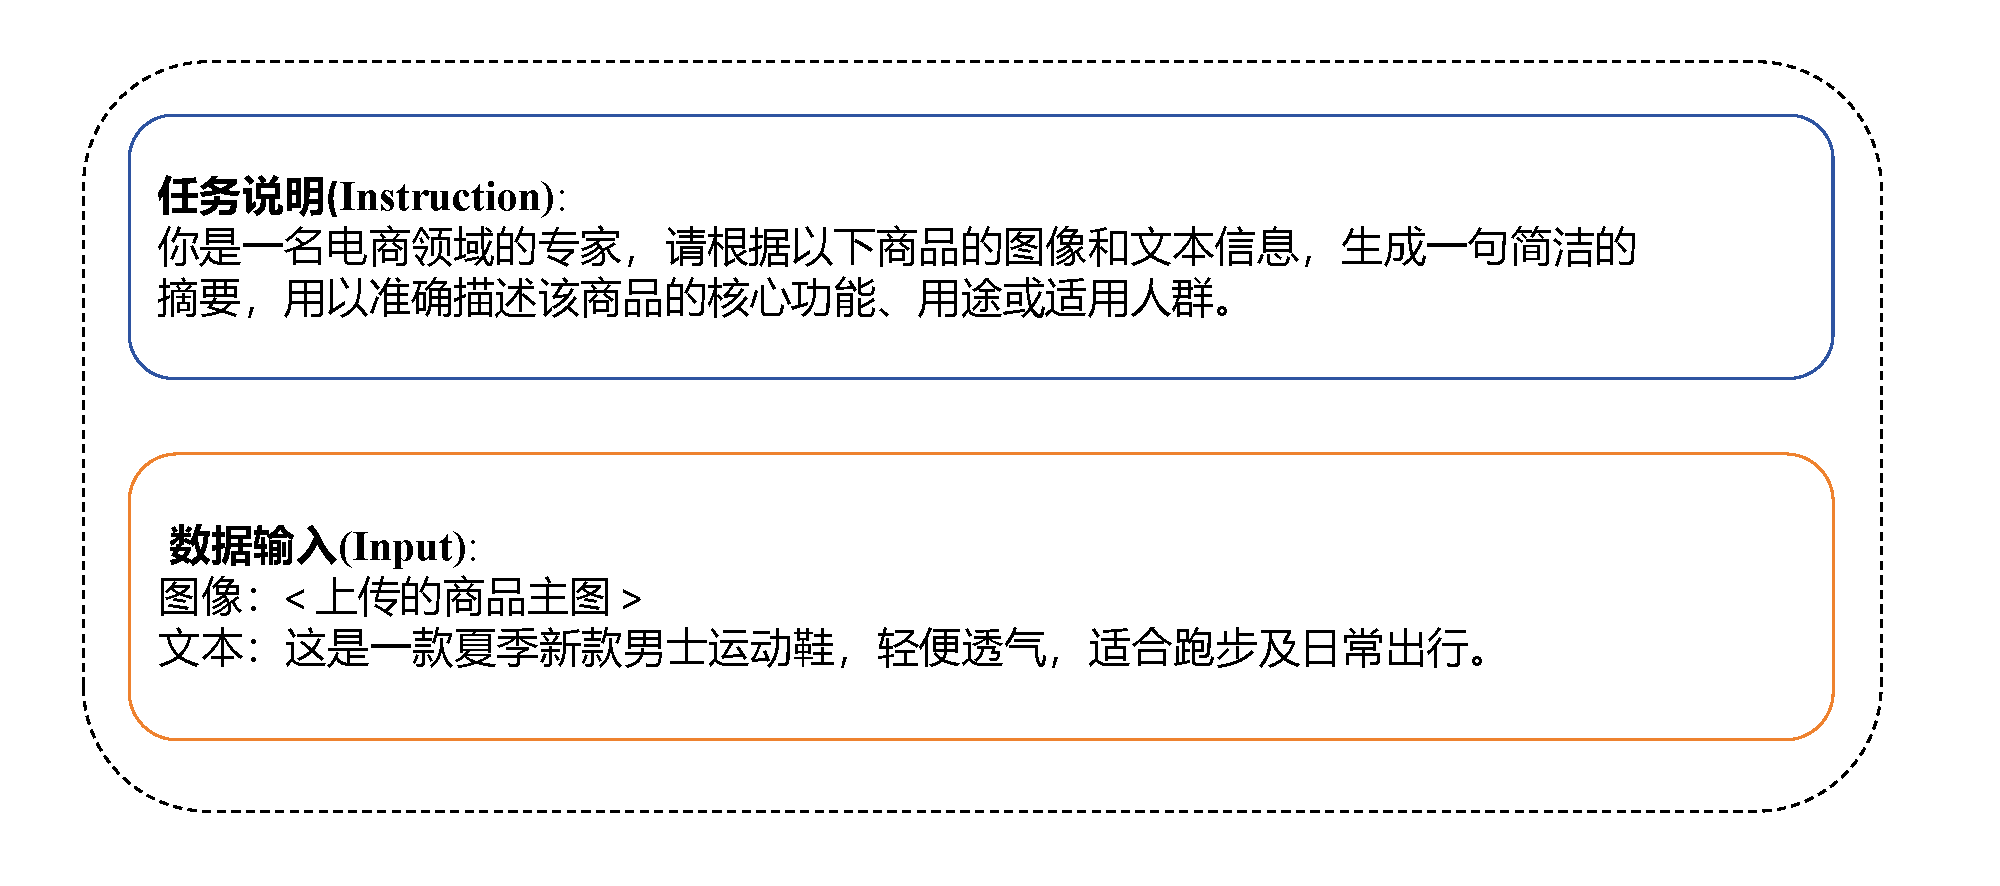
\includegraphics[width=1.0\textwidth]{figures/prompt1.pdf} 
\caption{物品摘要生成的 Prompt 模板示意图。}
\label{fig:prompt1}
\end{figure}


多模态大语言模型在接收上述输入后，将联合理解图像与文本两种模态的信息，并输出一段高语义浓度的商品摘要。例如：“轻质透气的男士跑步鞋，适合日常通勤与运动。”  
该摘要被记作物品的语义描述 $s_i$，用于后续的用户偏好建模与图结构构建。

\textbf{用户偏好摘要生成机制：}  
在获得所有物品的模态摘要后，结合用户的多行为交互记录生成用户的偏好摘要文本。对于每个用户，将其交互过的物品摘要文本、行为类型（如点击、加购、收藏、购买）以及交互评分一并输入 LLM。  
交互评分来源于前一工作 NIPER 所提出的基于因果推断的协同加权机制，该机制通过跨行为与行为内的加权计算，为每条用户–物品交互分配一个反映交互可靠性与强度的权重分值，从而量化不同交互行为的重要性。

为了引导 LLM 理解行为强度与语义内容之间的关系，从而生成能够反映稳定兴趣偏好的文本摘要，我们将设计的 Prompt 模板具体内容可视化如图~\ref{fig:prompt2} 所示。

\begin{figure}[h]
\centering
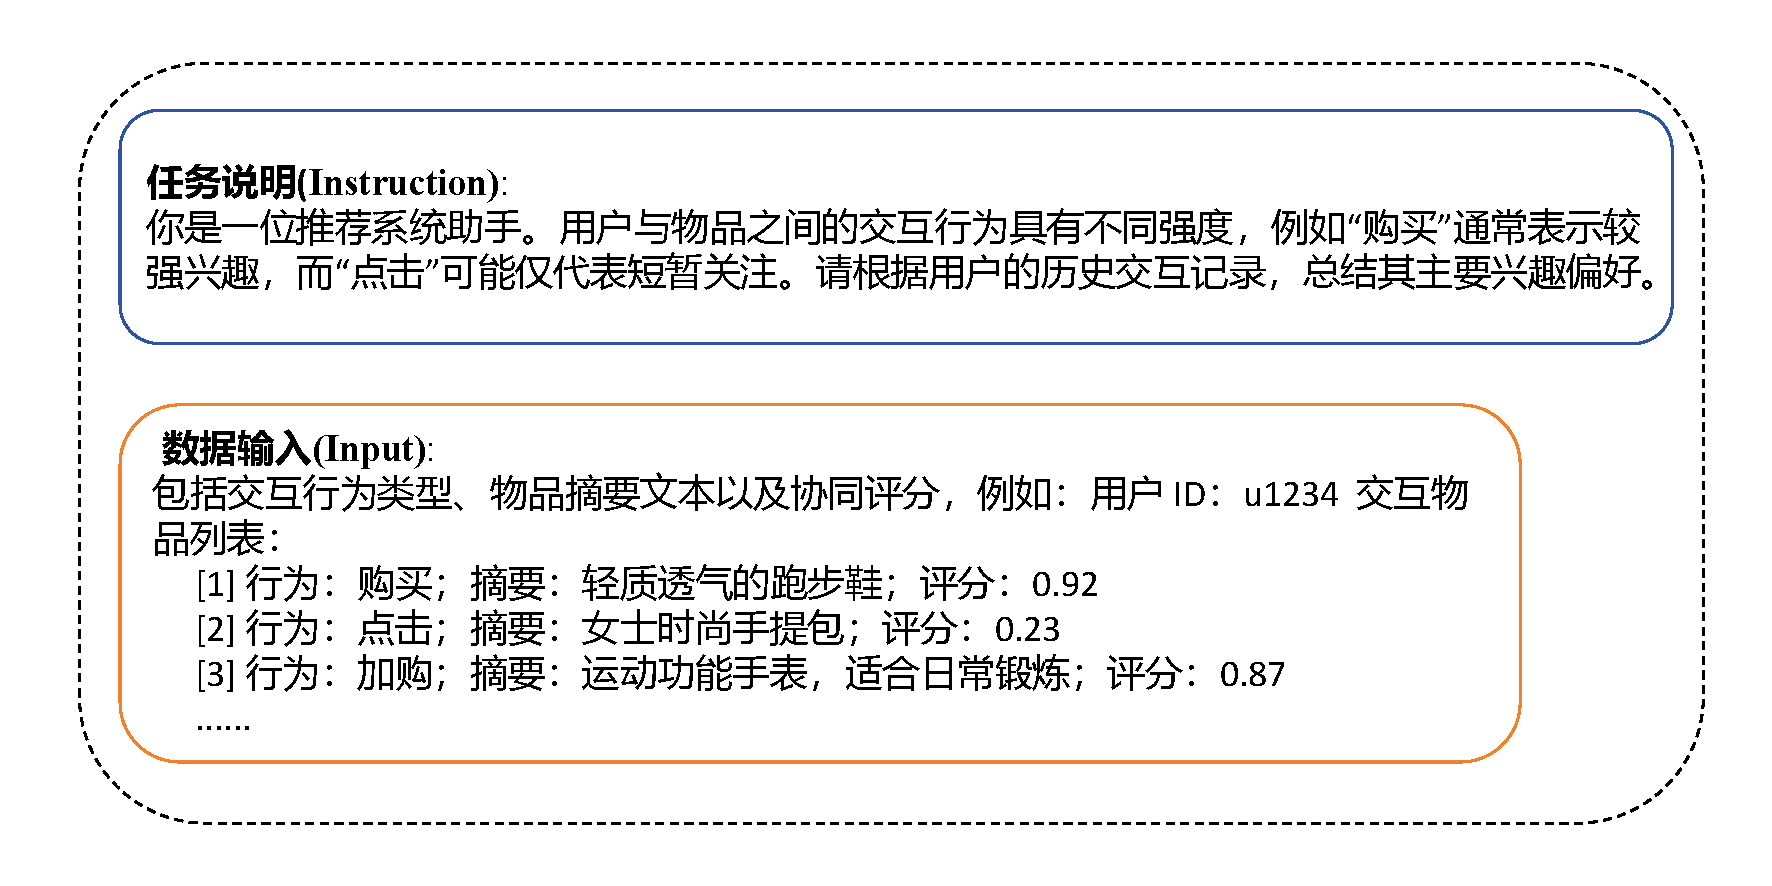
\includegraphics[width=1.0\textwidth]{figures/prompt2.pdf} 
\caption{用户偏好摘要生成的 Prompt 模板示意图。}
\label{fig:prompt2}
\end{figure}

LLM 在理解交互强度、协同评分与模态语义的关系后，生成概括性的用户偏好摘要文本 $s_u$，如“偏好运动休闲类商品，特别关注轻便跑鞋与户外装备”。  
在此基础上，利用生成的用户偏好文本与物品模态摘要文本构建统一的语义表示空间，以支持后续基于模态相似度的硬去噪机制。

\textbf{语义嵌入与基于相似度的硬去噪：}  
为获得用户与物品的语义表示，首先将用户偏好摘要文本 $s_u$ 与物品模态摘要文本 $s_i$ 输入预训练语言模型 BERT，得到高维原始模态语义向量：
\begin{equation}
\mathbf{h}_u = \mathrm{BERT}(s_u), \qquad
\mathbf{h}_i = \mathrm{BERT}(s_i).
\end{equation}

由于原始 BERT 表征 $\mathbf{h}$ 能完整保留语义细节，因此在识别辅助行为中的噪声交互时，直接使用 $\mathbf{h}_u$ 与 $\mathbf{h}_i$ 计算用户与其交互物品之间的语义相似度：
\begin{equation}
s_{ui} = \frac{\mathbf{h}_u^\top \mathbf{h}_i}{\|\mathbf{h}_u\|\,\|\mathbf{h}_i\|}.
\end{equation}
随后对每位用户的相似度得分进行 softmax 归一化：
\begin{equation}
\tilde{s}_{ui} = 
\frac{\exp(s_{ui}/\tau)}{\sum_{j \in \mathcal{I}_u} \exp(s_{uj}/\tau)},
\end{equation}
并根据阈值 $\delta$ 删除语义相关性较低的辅助行为交互（购买行为始终保留）：
\begin{equation}
\mathcal{G}_{\text{denoised}}
= \mathcal{G}^R \setminus
\{(u,i,b) \mid b \in \mathcal{B}_{\text{aux}},\, \tilde{s}_{ui} < \delta\}.
\end{equation}
该步骤基于未经投影的原始语义空间进行判断，从而避免降维带来的语义偏差影响噪声识别质量。

在得到去噪后的多行为交互图后，将用户与物品的模态表示输入多层感知机（MLP）进行投影与降维，使其与图神经网络得到的行为嵌入处于一致的向量尺度：
\begin{equation}
\widetilde{\mathbf{e}}_u = \mathrm{MLP}(\mathbf{h}_u), \qquad
\widetilde{\mathbf{e}}_i = \mathrm{MLP}(\mathbf{h}_i).
\end{equation}

为增强降维后的模态语义嵌入与 GNN 行为嵌入 $\mathbf{g}_u, \mathbf{g}_i$ 的表示一致性，引入基于余弦相似度的对齐正则项：
\begin{equation}
\mathcal{L}_{\text{align}}
= 1 - \frac{1}{|\mathcal{X}|}
\sum_{x \in \mathcal{X}}
\frac{\mathbf{g}_x^\top \widetilde{\mathbf{e}}_x}
{\|\mathbf{g}_x\| \, \|\widetilde{\mathbf{e}}_x\|},
\end{equation}
其中 $\mathcal{X}$ 表示用户与物品节点集合。该正则项最大化结构表示与模态表示的方向一致性，从而实现语义空间与行为空间的有效融合，同时避免了 KL 散度等分布对齐方法的数值不稳定性。

\section{语义感知注意力的软去噪消息传递}  
在获得去噪后的加权交互图 $\boldsymbol{G_{\mathrm{denoised},k}}$ 后，为进一步缓解残余噪声干扰并提升表示的语义一致性，本文引入带有语义引导的消息传递机制，实现基于注意力的软去噪（soft denoising）。该过程以图神经网络为核心，在 GHCF \cite{chen2021GHCF} 框架基础上，通过引入 Query–Key–Value（QKV） 注意力机制，动态调整邻居节点在信息聚合中的权重，从而抑制低语义相关的邻居贡献，强化与用户兴趣一致的高相关邻居信号。

不同于原始 GHCF 在各行为子图中对同类邻居进行等权聚合的方式，本研究根据用户与邻居物品在语义空间中的相似度自适应地分配聚合权重，使消息传递过程具备噪声感知能力。  
在第 $l$ 层传播中，首先将用户与物品的模态语义嵌入 $\widetilde{\mathbf{e}}_u$ 与 $\widetilde{\mathbf{e}}_v$ 分别映射为 Query 与 Key 表示，而 Value 向量来自邻居节点的交互嵌入 $\mathbf{e}_v^{(l)}$：
\begin{equation}
\mathbf{q}_u = \mathbf{W}_Q^{(l)} \widetilde{\mathbf{e}}_u, \quad
\mathbf{k}_v = \mathbf{W}_K^{(l)} \widetilde{\mathbf{e}}_v, \quad
\mathbf{v}_v^{(l)} = \mathbf{W}_V^{(l)} \mathbf{e}_v^{(l)},
\end{equation}
其中，$\mathbf{W}_Q^{(l)}$、$\mathbf{W}_K^{(l)}$ 和 $\mathbf{W}_V^{(l)}$ 为第 $l$ 层的可学习参数矩阵。

随后，用户 $u$ 与其邻居物品 $v \in N_{u,k}$ 的注意力权重基于语义相关性计算得到：
\begin{equation}
\alpha^{(l)}_{uv,k} =
\mathrm{softmax}\!\left(
\frac{\mathbf{q}_u^\top \mathbf{k}_v}{\sqrt{d}}
\right)_{v \in N_{u,k}},
\end{equation}
其中 $d$ 为嵌入维度。该权重反映了邻居节点在语义空间中与用户兴趣的一致程度，高相似度邻居在聚合中获得更大权重，而语义不一致的噪声邻居则被自然削弱，从而实现了隐式的软去噪。

基于注意力权重，对邻居节点的特征进行加权聚合，得到用户 $u$ 在行为 $k$ 下的更新表示：
\begin{equation}
\mathbf{e}^{(l+1)}_{u,k} =
\mathrm{LeakyReLU}\!\left(
\mathbf{W}^{(l)}
\sum_{v \in N_{u,k}}
\alpha^{(l)}_{uv,k}
\left(
\mathbf{v}_v^{(l)} \odot \mathbf{e}_k^{(l+1)}
\right)
\right),
\end{equation}
其中，$\odot$ 表示逐元素乘，$\mathbf{e}_k^{(l+1)}$ 为行为类型的嵌入，$\mathbf{W}^{(l)}$ 为特征变换矩阵。

为了进一步建模行为类型间的差异性，对每种行为类型嵌入进行线性变换：
\begin{equation}
\mathbf{e}_k^{(l+1)} = \mathbf{W}_b^{(l)} \mathbf{e}_k,
\end{equation}
其中 $\mathbf{W}_b^{(l)}$ 为行为特征映射矩阵。最终，经过多层传播后，可分别得到用户嵌入 $E_u$、物品嵌入 $E_v$ 和行为类型嵌入 $E_k$，其中 $k \in \mathcal{B}$ 为行为集合。

该语义感知注意力机制通过在消息传递过程中显式建模用户与邻居间的语义相关性，实现了对残余噪声的软抑制（soft denoising），使模型能够在多模态多行为场景下学习到更加鲁棒且语义一致的用户与物品表示。


\section{模态感知图增强与对比学习}
\textbf{语义增强图构建：}  
为缓解原始交互图中真实偏好边的缺失问题，并进一步发挥模态语义在推荐任务中的补充作用，构建了基于模态一致性的语义增强图 $\mathcal{G}_{\mathrm{aug}}$。该图以辅助行为图（即 $G^R_k, \; k = 1, \ldots, K-1$）为基础，通过筛选语义一致性较高的用户–物品交互对来补充目标行为图 $G^R_K$，从而在保持协同结构的同时引入内容层面的关联信息。

具体而言，基于用户与物品的模态语义嵌入 $\widetilde{\mathbf{e}}_u$ 与 $\widetilde{\mathbf{e}}_v$，采用余弦相似度衡量二者的语义相关性：
\begin{equation}
\mathrm{sim}(u, v) = 
\frac{
\widetilde{\mathbf{e}}_u^\top \widetilde{\mathbf{e}}_v
}{
\|\widetilde{\mathbf{e}}_u\| \, \|\widetilde{\mathbf{e}}_v\|
}.
\end{equation}
当 $\mathrm{sim}(u, v)$ 超过设定阈值 $\beta$ 时，认为该辅助行为交互在语义上可能反映了用户的真实兴趣意图，因此将其纳入语义增强图：
\begin{equation}
\mathcal{G}_{\mathrm{sim}} =
\left\{
(u, v)
\mid
\exists k \in \{1, \ldots, K-1\},\;
(u, v) \in G^R_k,\;
\mathrm{sim}(u, v) > \beta
\right\}.
\end{equation}
最终，语义增强图 $\mathcal{G}_{\mathrm{sim}}$ 被并入目标行为图，形成增强后的目标行为图：
\begin{equation}
\widetilde{G}^R_K = G^R_K \cup \mathcal{G}_{\mathrm{sim}},
\end{equation}
并将其与原始辅助行为图集合共同记为 $\mathcal{G}_{\mathrm{aug}}$。  
该增强策略通过引入高置信度的模态语义边补充协同图的结构信息，有效提升了目标行为图对用户真实兴趣的刻画能力。

\textbf{跨图表示对比学习：}  
为进一步实现语义增强图 $\mathcal{G}_{\mathrm{aug}}$ 与去噪图 $\mathcal{G}_{\mathrm{denoised}}$ 之间的知识迁移与偏好一致性建模，引入了跨图对比学习（cross-graph contrastive learning）策略。该机制利用模态信息生成正负样本对，从语义视角对齐两图中的节点表示，促进语义信息的高效传递。

具体而言，将两张图分别输入图神经网络（GNN），得到用户与物品在两种图结构下的嵌入表示：
\begin{equation}
\mathbf{e}_u, \mathbf{e}_v = \mathrm{GNN}(\mathcal{G}_{\mathrm{denoised}}), \quad
\mathbf{e}_u^{\mathrm{aug}}, \mathbf{e}_v^{\mathrm{aug}} = \mathrm{GNN}(\mathcal{G}_{\mathrm{aug}}).
\end{equation}
其中，$\mathbf{e}_u$ 与 $\mathbf{e}_v$ 分别为去噪图中用户与物品的嵌入，$\mathbf{e}_u^{\mathrm{aug}}$ 与 $\mathbf{e}_v^{\mathrm{aug}}$ 则来自语义增强图。

为强化两种图视角下的语义一致性，对同一节点在两图中的嵌入施加对比学习约束。以用户为例，对比学习损失定义为：
\begin{equation}
\mathcal{L}_{\mathrm{contrast}}^{(u)} =
- \log
\frac{
\exp\!\left(
\cos(\mathbf{e}_u, \mathbf{e}_u^{\mathrm{aug}}) / \tau
\right)
}{
\sum\limits_{u' \in \mathcal{U}}
\exp\!\left(
\cos(\mathbf{e}_u, \mathbf{e}_{u'}^{\mathrm{aug}}) / \tau
\right)
},
\end{equation}
其中 $\tau$ 为温度系数，$\cos(\cdot)$ 表示余弦相似度。  
同理，物品端的对比损失为：
\begin{equation}
\mathcal{L}_{\mathrm{contrast}}^{(v)} =
- \log
\frac{
\exp\!\left(
\cos(\mathbf{e}_v, \mathbf{e}_v^{\mathrm{aug}}) / \tau
\right)
}{
\sum\limits_{v' \in \mathcal{I}}
\exp\!\left(
\cos(\mathbf{e}_v, \mathbf{e}_{v'}^{\mathrm{aug}}) / \tau
\right)
}.
\end{equation}
最终的跨图对比学习目标定义为：
\begin{equation}
\mathcal{L}_{\mathrm{contrast}} =
\mathcal{L}_{\mathrm{contrast}}^{(u)} +
\mathcal{L}_{\mathrm{contrast}}^{(v)}.
\end{equation}

该模块利用模态信息构建正负样本对，将语义增强图中的高质量语义关系显式传递至去噪图的节点表示中，从而在结构空间与语义空间间实现信息对齐，显著提升用户与物品嵌入的鲁棒性与泛化能力。


\section{模型训练}
为实现多模态多行为场景下的稳定训练与鲁棒优化，模型的最终目标函数综合考虑了推荐精度、语义一致性与跨图表示对齐三方面因素。

首先，推荐损失仍采用与第一部分 NIPER 相同的非采样优化形式，用于直接回归用户–物品交互概率，避免负采样引入的噪声误差。对于特定用户批次 $B$ 与整个物品集合 $\mathcal{I}$，行为 $k$ 下的非采样推荐损失定义为：
\begin{equation}
\mathcal{L}_{\mathrm{rec}}^{k}
= 
\sum_{u \in B} \sum_{i \in I_u^{k+}}
\left[
\left(c_i^{k+} - c_i^{k-}\right)
\left(\hat{x}_{u,i}^k\right)^2
-
2 c_i^{k+} \hat{x}_{u,i}^k
\right],
\end{equation}
其中，$\hat{x}_{u,i}^k$ 表示用户 $u$ 在行为 $k$ 下对物品 $i$ 的预测偏好值，
$ I_u^{k+} $ 为正交互集合，$ c_i^{k+} $ 与 $ c_i^{k-} $ 为经验超参数。

整体推荐损失为各行为损失的加权和：
\begin{equation}
\mathcal{L}_{\mathrm{rec}} = 
\sum_{k=1}^{K} \lambda_k \mathcal{L}_{\mathrm{rec}}^{k},
\end{equation}
其中 $\lambda_k$ 表示第 $k$ 种行为的权重。

其次，为实现语义增强图与去噪图之间的信息传递与偏好一致性，引入跨图对比学习损失：
\begin{equation}
\mathcal{L}_{\mathrm{contrast}} =
\mathcal{L}_{\mathrm{contrast}}^{(u)} +
\mathcal{L}_{\mathrm{contrast}}^{(v)},
\end{equation}
其中用户端与物品端的对比损失定义为：
\begin{equation}
\mathcal{L}_{\mathrm{contrast}}^{(u)} =
- \log
\frac{
\exp\!\left(
\cos(\mathbf{e}_u, \mathbf{e}_u^{\mathrm{aug}}) / \tau
\right)
}{
\sum\limits_{u' \in \mathcal{U}}
\exp\!\left(
\cos(\mathbf{e}_u, \mathbf{e}_{u'}^{\mathrm{aug}}) / \tau
\right)
},
\quad
\mathcal{L}_{\mathrm{contrast}}^{(v)} =
- \log
\frac{
\exp\!\left(
\cos(\mathbf{e}_v, \mathbf{e}_v^{\mathrm{aug}}) / \tau
\right)
}{
\sum\limits_{v' \in \mathcal{I}}
\exp\!\left(
\cos(\mathbf{e}_v, \mathbf{e}_{v'}^{\mathrm{aug}}) / \tau
\right)
}.
\end{equation}

此外，为防止 MLP 降维造成的语义漂移，引入余弦一致性正则项，用以保持投影后嵌入与GNN学习的协同侧嵌入的语义方向一致：
\begin{equation}
\mathcal{L}_{\mathrm{align}} =
1 -
\frac{1}{|\mathcal{X}|}
\sum_{x \in \mathcal{X}}
\frac{
\mathbf{h}_x^\top \widetilde{\mathbf{e}}_x
}{
\|\mathbf{h}_x\| \, \|\widetilde{\mathbf{e}}_x\|
},
\end{equation}
其中 $\mathcal{X}$ 为用户与物品节点的集合。

最终的联合优化目标定义为：
\begin{equation}
\mathcal{L} =
\mathcal{L}_{\mathrm{rec}}
+
\mu \, \mathcal{L}_{\mathrm{contrast}}
+
\gamma \, \mathcal{L}_{\mathrm{align}},
\end{equation}
其中，$\mu$ 与 $\gamma$ 分别为对比学习与语义一致性正则项的权重系数。

在优化完成后，用户 $u$ 对物品 $v$ 的目标行为预测概率为：
\begin{equation}
\hat{y}_{uv}^{(k)} =
\mathbf{e}_u^\top
\cdot
\mathrm{diag}(\mathbf{e}_k)
\cdot
\mathbf{e}_v,
\end{equation}
其中 $\mathbf{e}_u$、$\mathbf{e}_v$ 分别为用户与物品嵌入，
$\mathbf{e}_k$ 为目标行为类型的嵌入向量，
$\mathrm{diag}(\mathbf{e}_k)$ 表示以 $\mathbf{e}_k$ 为对角元素的对角矩阵。

该联合目标在优化过程中同时约束了结构信号、模态语义与跨图一致性，从而实现了鲁棒、稳健的多模态多行为去噪推荐建模。

\section{实验与讨论}

\subsection{评价指标}
为全面评估模型的推荐性能，本文采用命中率（Hit Ratio，HR）与归一化折损累计增益（Normalized Discounted Cumulative Gain，NDCG）作为主要评价指标，其计算方式与第三章相同。
其中，HR 用于衡量模型在前 $K$ 个推荐结果中命中目标物品的比例，反映模型的召回能力；NDCG 则综合考虑目标物品在推荐列表中的排名位置，更能体现推荐结果的排序合理性与相关性。

\subsection{数据集信息}
由于第三章所使用的数据集仅包含用户与物品在多种行为下的交互信息（如点击、加购、购买等），缺乏文本与图像等模态特征，无法支撑多模态场景下的去噪与偏好建模研究。为进一步扩展模型至多模态多行为推荐任务，本章基于 Tmall 平台的原始数据重新构建了一个多模态多行为推荐数据集——\textbf{Tmall-Rec}\footnote{https://tianchi.aliyun.com/dataset/140281}。  
该数据集在保留用户–物品多行为交互关系的基础上，补充了物品侧的文本描述与图像信息，使得模型能够同时利用协同交互信号与多模态内容特征进行联合建模，从而更深入地探索用户真实偏好识别与噪声过滤机制。表~\ref{tab:dataset2} 展示了该数据集的统计信息。

\begin{table}[h]
\centering
\caption{Tmall-Rec 数据集的统计信息}
\renewcommand{\arraystretch}{1.0}
\label{tab:dataset2}
\scalebox{0.9}{
\begin{tabular}{cccccc}
\toprule
数据集 & \#User & \#Item & \#View & \#Cart & \#Buy \\
\midrule
Tmall-Rec & 8,302 & 30,316 & 496,615 & 60,798 & 43,172 \\
\bottomrule
\end{tabular}
}
\end{table}

\subsection{实验设置}
实验基于 PyTorch 实现，优化器采用 Adam，学习率设为 0.001，批量大小为 256。图神经网络（GNN）的嵌入维度为 64；为缓解过拟合，训练中使用嵌入丢弃率 0.3 与边丢弃率 0.1。非采样推荐目标的负样本权重固定为 0.01。对比学习的温度系数 $\tau$ 在区间 $[0.1, 0.5]$ 内网格搜索。文本语义编码器采用 Sentence-BERT，其输出维度为 768；随后通过一个 MLP 投影到 64 维以与 GNN 表示空间对齐并降低计算开销。多模态摘要与语义对齐由 Qwen-2.5-VL-72B 完成，输入为物品图像与标题以及用户的多行为交互信息。

\subsection{总体实验效果}

\begin{table*}[htbp]
\renewcommand{\arraystretch}{1.0}
\caption{Tmall-Rec 数据集上各模型的性能比较结果}
\centering
\begin{tabular}{l|cccc}
\toprule
\multirow{2}{*}{Model} & \multicolumn{4}{c}{Tmall-Rec}  \\
& Recall@5 & Recall@10 & NDCG@5 & NDCG@10 \\
\midrule
LightGCN~\cite{he2020lightgcn} & 0.0823 & 0.2049 & 0.0742 & 0.1598 \\
FREEDOM~\cite{zhou2023tale} & 0.1874 & 0.3412 & 0.1438 & 0.2487 \\
GHCF~\cite{chen2021GHCF} & 0.3117 & 0.4079 & 0.2274 & 0.2585 \\
DPT~\cite{zhang2023DPT} & 0.3571 & 0.4762 & 0.2745 & 0.3017 \\
MBSSL~\cite{xu2023MBSSL} & 0.3934 & 0.5063 & 0.2932 & 0.3298 \\
\textbf{Ours} & \textbf{0.5064} & \textbf{0.5925} & \textbf{0.3973} & \textbf{0.4253} \\ 
\bottomrule
\end{tabular}
\label{table:Comparison2} 
\end{table*}

为验证所提多模态多行为去噪推荐算法的有效性，本章与三类具有代表性的推荐模型进行了系统对比，具体如下：
\textbf{单行为推荐模型（Single-Behavior Recommendation Models）。}
该类方法仅基于目标行为进行建模，用于评估多行为协同建模带来的性能提升。代表模型包括经典协同过滤方法 LightGCN~\cite{he2020lightgcn}。

\textbf{多模态推荐模型（Multi-Modal Recommendation Models）。}
以及融合模态特征的单行为多模态推荐模型 FREEDOM~\cite{zhou2023tale}。

\textbf{去噪推荐模型（Denoising Recommendation Models）。}
此类方法通过识别和抑制噪声交互以提升推荐结果的鲁棒性。本文选取多行为场景下具有代表性的去噪方法 DPT~\cite{zhang2023DPT} 作为对比模型。

\textbf{多行为推荐模型（Multi-Behavior Recommendation Models）。}
该类方法显式建模多种用户行为间的相关性，以增强目标行为的预测能力。本文选取 GHCF~\cite{chen2021GHCF} 与基于自监督机制的 MBSSL~\cite{xu2023MBSSL} 作为代表性多行为推荐模型进行对比。

表~\ref{table:Comparison2} 展示了多模态多行为去噪推荐算法与三类基线模型在 Tmall-Rec 数据集上的综合性能比较结果。  
所有模型均采用在验证集上表现最优的超参数配置进行评估，以确保结果的公平性。

从整体结果来看，所提算法在 Recall@K 与 NDCG@K 等主要指标上均取得了显著提升，表现出更优的推荐准确性与排序能力。  
其中，在 Recall@10 和 NDCG@10 上，较当前表现最优的多行为模型 MBSSL 分别提升约 12\% 与 10\%，在各评价指标上均保持领先。

从模型结构角度分析，传统单行为模型（如 LightGCN）由于未考虑多行为信号之间的关联，仅能学习目标行为层面的偏好模式，整体性能较低。  
加入模态特征的 FREEDOM 在一定程度上提升了内容表达能力，但其缺乏对多行为协同关系与噪声交互的建模，仍存在语义偏差与过拟合问题。  
多行为推荐方法 GHCF 与 MBSSL 能够捕获行为间的关联性，从而在多源交互数据上获得更优表现，但其对多模态内容的利用较为有限，且在存在噪声干扰的场景中表现下降。

相比之下，所提算法在两方面实现了显著优势：  
（1）通过引入大模型生成的模态语义摘要，有效弥补了协同信号中缺失的内容信息，使模型能够在语义空间中对齐用户与物品的真实偏好关系；  
（2）结合基于模态相似度的硬去噪机制与语义感知的软去噪聚合策略，显著降低了辅助行为中随机性与非兴趣驱动交互的干扰，确保图结构中保留的信息更加纯净。

综合来看，该算法在多模态融合与噪声抑制两方面均展现出较高的鲁棒性与表达能力，验证了在复杂交互场景下引入模态语义信息与分层去噪机制的必要性与有效性。

为确保实验结果的可靠性，本研究中的所有实验均重复执行 5 次，每次实验仅改变随机种子（seed），其余超参数和训练设置保持一致。对于每次实验，我们记录关键评价指标，并计算其均值与标准差。结果显示，不同随机种子对模型性能的波动较小，标准差约为指标均值的 $1.4\%$ 左右，表明方法具有较高的稳定性。

针对主要指标，本文采用 Wilcoxon 符号秩检验（Wilcoxon signed-rank test）进行显著性分析，以验证本文方法相较于基线方法的性能提升是否具有统计意义。实验结果显示，关键指标的 $p$ 值远小于 $0.05$，表明性能提升具有统计显著性。通过重复实验、方差分析及显著性检验，本研究能够有效排除偶然因素的影响，为多行为推荐方法的性能评估提供可靠依据。

\subsection{消融实验}
为验证所提出模型中各个设计模块的有效性与必要性，本节进行了系统的消融实验。具体地，设计了以下四个模型变体：

\begin{enumerate}
    \item \textbf{GNN only：} 仅保留基础的 GHCF 网络结构，对多行为交互进行建模，不引入任何模态或去噪模块；
    \item \textbf{w/o 硬去噪：} 移除基于多模态信息的硬去噪模块，保留语义感知消息传递与对比学习；
    \item \textbf{w/o 软去噪：} 移除语义感知注意力机制，使用与 GHCF 相同的均值聚合方式进行消息传递；
    \item \textbf{w/o 硬打分：} 移除基于多模态信息的硬去噪模块中的用户-物品交互打分，在大模型的输入中将同等行为视为同等权重；
    \item \textbf{w/o SSL：} 移除模态感知图增强与跨图对比学习模块，仅保留去噪与基本 GNN 表示学习；
\end{enumerate}

消融实验结果如表~\ref{table:ablation2} 所示。结果分析如下：

\textbf{基础 GNN 的性能对比。}  
与完整模型相比，仅使用 GHCF 结构（\textbf{GNN only}）的性能显著较低，说明单纯依赖协同信号难以充分建模用户的真实偏好。  
这验证了引入多模态语义与去噪机制对于提升表示质量与缓解交互噪声具有重要意义。

\textbf{硬去噪机制的重要性。}  
移除硬去噪模块后，模型性能显著下降，表明多模态信息在识别和剔除非真实交互方面发挥了关键作用。  
硬去噪模块通过计算用户与物品在语义空间中的模态相似度，有效过滤了语义不一致或低相关的辅助行为交互，从而降低了噪声干扰。  
当该机制被移除时，噪声交互被直接用于训练，导致表示学习受污染，用户偏好建模的准确性显著下降。

\textbf{软去噪模块的必要性。}  
替换语义感知注意力为均值聚合后，模型在所有评估指标上均出现明显退化，表明软去噪机制在信息传播过程中的自适应调节能力至关重要。  
基于语义相似度的注意力权重能够动态调整邻居节点的影响力，使模型在特征聚合时更关注语义一致性高的交互关系，从而提升用户与物品表示的判别性与稳定性。

\textbf{硬打分模块的有效性。}  
移除硬打分模块后，模型将所有用户–物品交互行为赋予同等权重，导致噪声干扰下推荐性能显著下降。该结果不仅验证了该模块在交互质量量化中的关键作用，更凸显其跨工作的强泛化能力：作为本论文第一项工作 NIPER 的核心组件，该机制在第二项工作中仍发挥关键作用。性能退化表明，该模块并非面向单一任务的定制设计，而是具备普适性的噪声感知基础单元，为多行为推荐系统提供了可迁移、可复用的交互质量评估范式。

\textbf{对比学习的有效性。}  
移除跨图对比学习模块后，模型泛化性能明显下降，验证了该模块在语义增强图与去噪图之间建立一致性约束的作用。  
对比学习通过在两个视角下对齐节点表示，促进了语义信息向结构空间的有效迁移，从而在保持表达一致性的同时增强了模型的鲁棒性。

\begin{table}[h]
\centering
\caption{消融实验结果（Tmall-Rec 数据集）}
\scalebox{0.9}{
\begin{tabular}{lcccc}
\toprule
\multirow{2}{*}{Model} & \multicolumn{4}{c}{Tmall-Rec} \\
\cmidrule(r){2-5}
 & Recall@5 & Recall@10 & NDCG@5 & NDCG@10 \\
\midrule
GNN only & 0.2902 & 0.3857 & 0.2098 & 0.2405 \\
w/o 硬去噪 & 0.4386 & 0.5337 & 0.3157 & 0.3444 \\
w/o 软去噪 & 0.4628 & 0.5835 & 0.3321 & 0.3695 \\
w/o 硬打分 & 0.4823 & 0.5599 & 0.3171 & 0.3489 \\
w/o SSL & 0.4409 & 0.5748 & 0.3279 & 0.3528 \\
\textbf{Ours} & \textbf{0.5064} & \textbf{0.5925} & \textbf{0.3973} & \textbf{0.4253} \\
\bottomrule
\end{tabular}
}
\label{table:ablation2}
\end{table}


\subsection{参数实验}

\begin{figure}[htbp]
    \centering
    % 第一行
    \begin{minipage}[t]{0.4\textwidth}
        \centering
        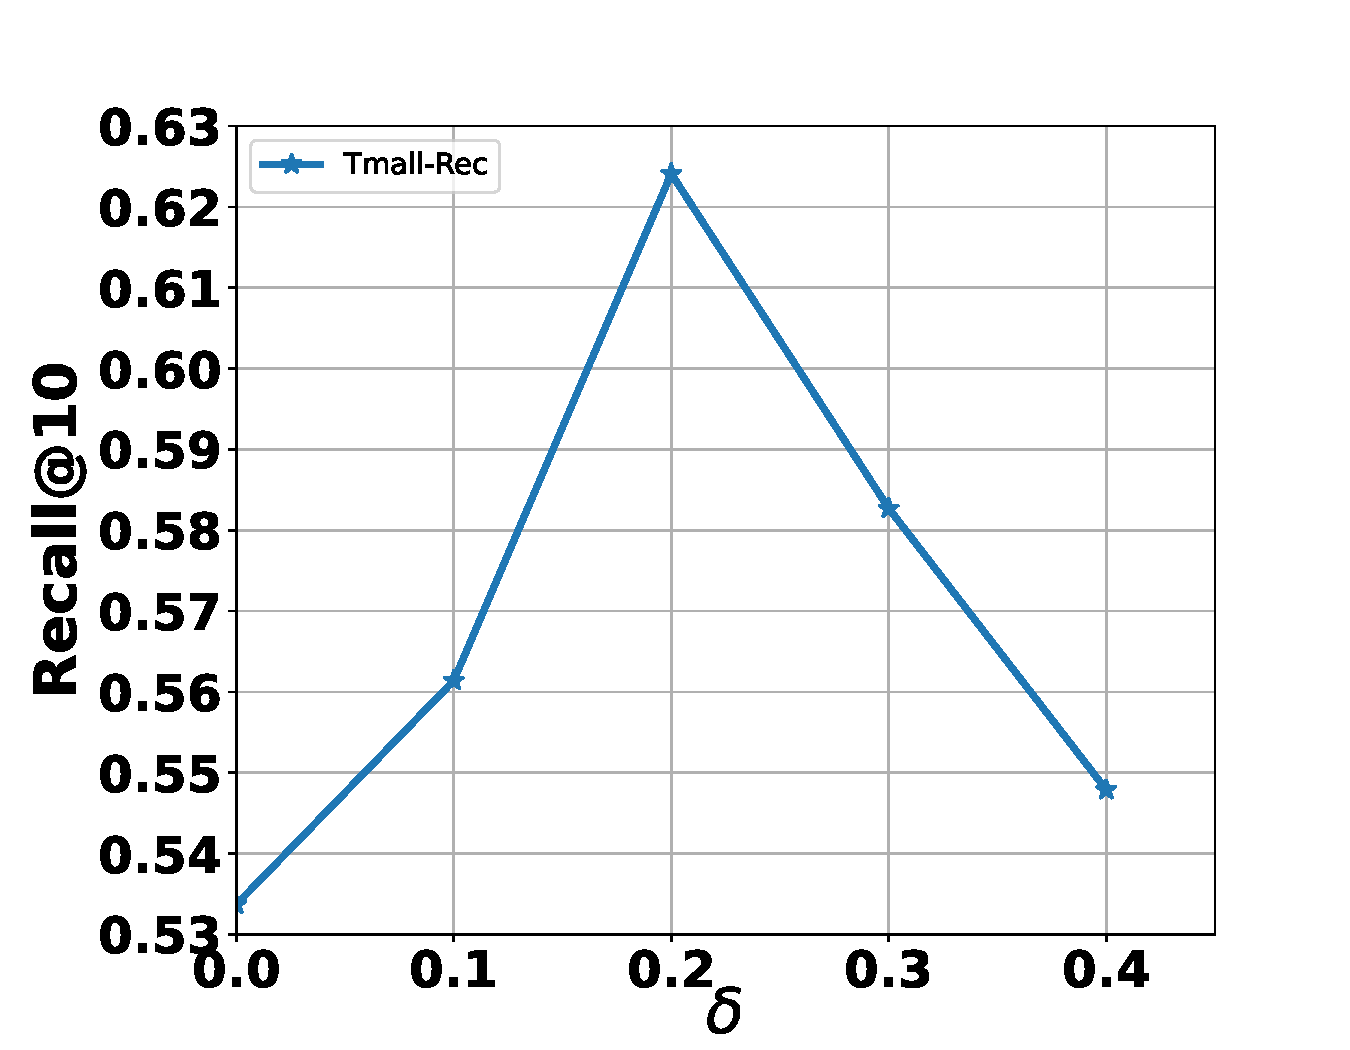
\includegraphics[width=\linewidth]{figures/delta.pdf}
        \caption*{\small (a) 硬噪声阈值 $\delta$}
    \end{minipage}
    \hspace{0.05\textwidth}
    \begin{minipage}[t]{0.4\textwidth}
        \centering
        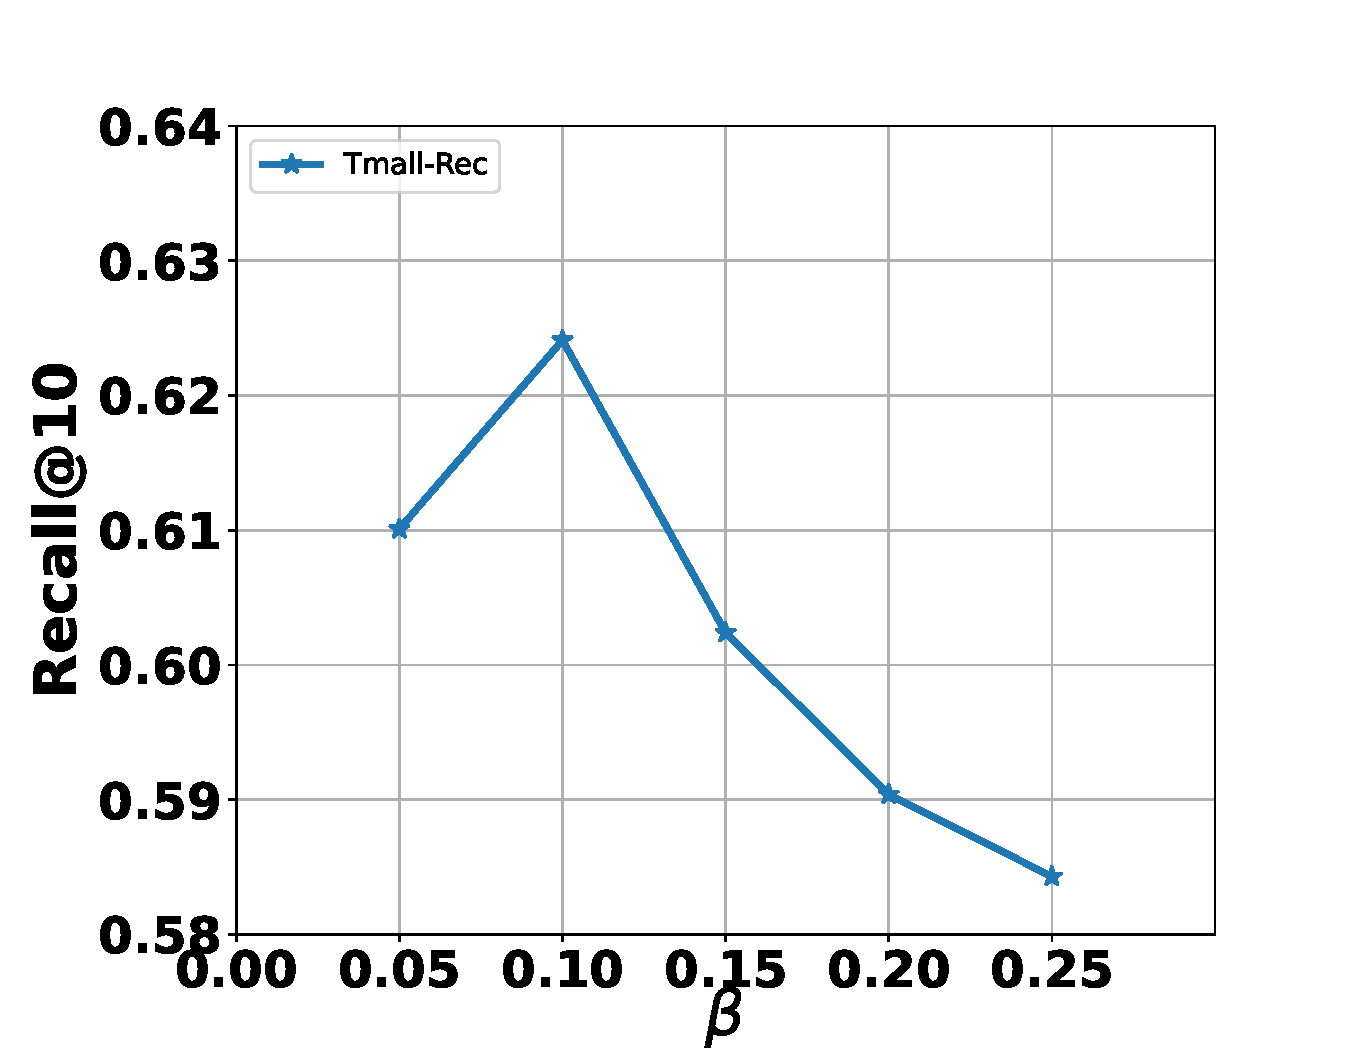
\includegraphics[width=\linewidth]{figures/beta.pdf}
        \caption*{\small (b) 语义增强阈值 $\beta$}
    \end{minipage}
    % 第二行
    \begin{minipage}[t]{0.4\textwidth}
        \centering
        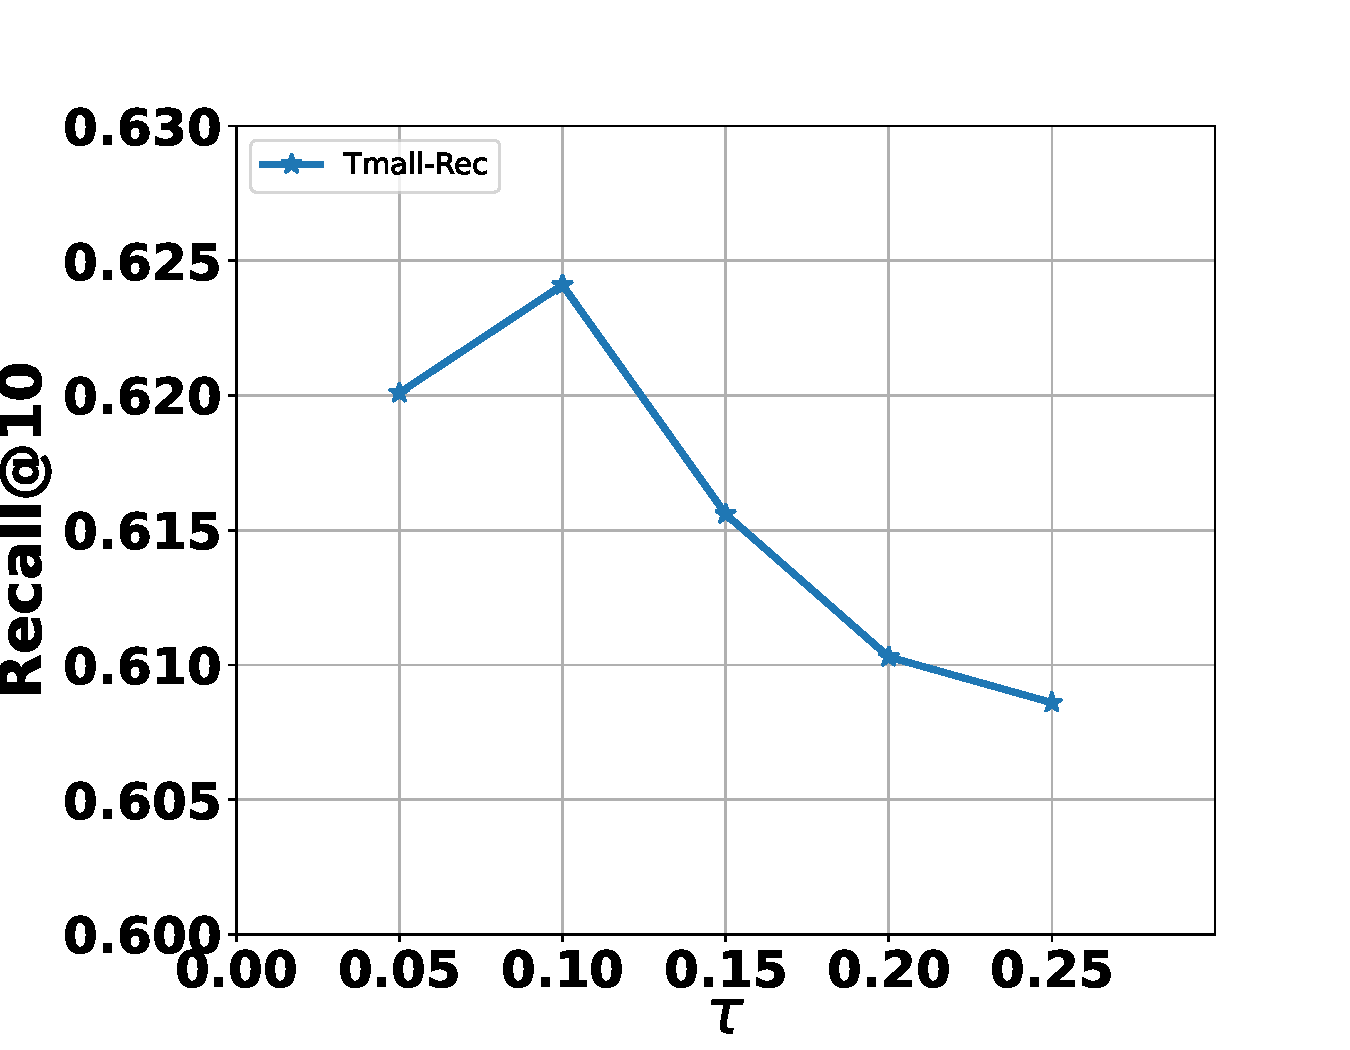
\includegraphics[width=\linewidth]{figures/temp.pdf}
        \caption*{\small (c) 对比学习温度系数 $\tau$}
    \end{minipage}
    \hspace{0.05\textwidth}
    \caption{超参数实验}
    \label{fig:para2}
\end{figure}


为系统分析模型关键超参数对整体性能的影响，本节从三个方面展开实验研究：硬噪声阈值 $\delta$、语义增强阈值 $\beta$ 以及对比学习温度系数 $\tau$。  
图~\ref{fig:para2} 展示了不同参数取值下模型在主要指标上的性能变化趋势。

\textbf{硬噪声阈值 $\delta$ 的影响：}  
该参数用于控制硬去噪阶段中交互样本的过滤强度。当阈值较低时，模型可能保留部分噪声样本，导致表示学习受到干扰；而当阈值过高时，真实但罕见的偏好交互可能被误删，造成信息损失。实验结果表明，适中的阈值能在噪声抑制与信息保留之间取得良好平衡，从而实现最优性能。

\textbf{语义增强阈值 $\beta$ 的影响：}  
语义增强阈值决定了辅助行为交互是否可被纳入语义增强图中。较低的阈值会引入更多低相关的辅助样本，降低图结构的纯度；较高的阈值则导致增强边数量不足，语义补充效果减弱。实验结果显示，适当提升 $\beta$ 能有效强化语义一致性，提升模型在高阶兴趣建模中的表现。

\textbf{对比学习温度系数 $\tau$ 的影响：}  
温度系数调节了对比学习中正负样本分布的平滑程度。当 $\tau$ 过大时，样本差异被弱化，导致对比约束不足；当 $\tau$ 过小时，梯度过于尖锐，模型训练不稳定。结果表明，适中的温度系数能兼顾表示区分性与优化稳定性，从而提升跨图对齐效果。

\subsection{案例研究}

\begin{figure}
\centering
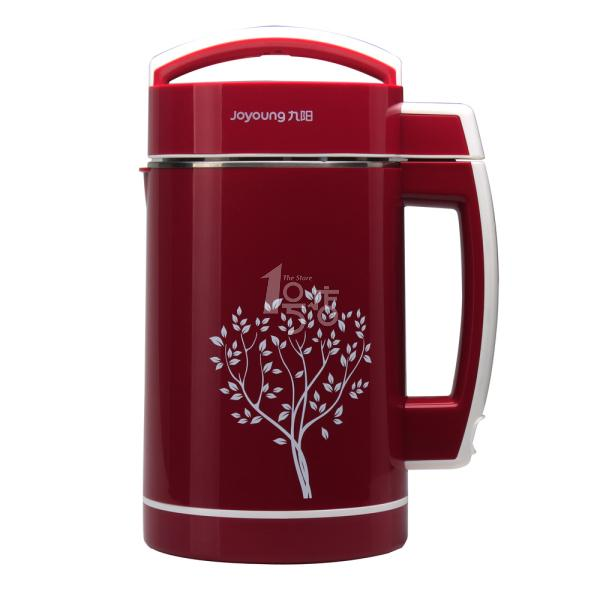
\includegraphics[width=0.36\linewidth]{figures/soymilk_maker.jpg}
\hspace{2mm}
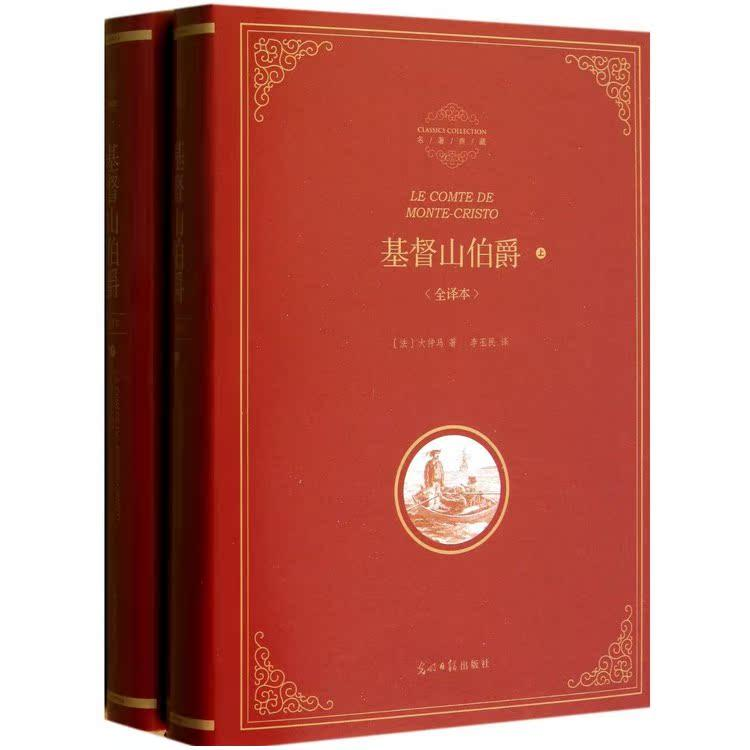
\includegraphics[width=0.36\linewidth]{figures/red_book.jpg}\\[2mm]
\begin{tabular}{l c}
\toprule
特征类型 & 相似度 \\
\midrule
视觉特征（Vision-only） & 0.57 \\
原始文本特征（Original Text） & 0.41 \\
LLM 增强文本特征（LLM-Enhanced Text） & \textbf{0.32} \\
\bottomrule
\end{tabular}
\caption{红色豆浆机与红色图书样本对在不同特征表征下的语义相似度。}
\label{fig:case_study}
\end{figure}

为验证本文提出的大模型模态增强方法在区分视觉相似但语义不同商品时的有效性，本节选取两张在视觉上高度相似、背景一致的商品图片（红色豆浆机与红色图书）构建案例对。两张图片在颜色、光照与构图上几乎一致，低层视觉特征高度相似，难以通过视觉表征区分。

实验对比了三种不同表征方式的相似度。如图~\ref{fig:case_study} 所示，视觉特征的相似度最高（0.57），表明传统视觉模型主要受颜色与外观影响；原始文本表征的相似度下降至 0.41，反映了文本语义对类别差异的初步区分；而本文提出的 LLM 增强文本方法进一步将相似度降低至 0.32，说明通过大语言模型生成的结构化语义描述（包含品类、功能、品牌等关键槽位信息），能够显著强化语义可分性，减少视觉共性带来的混淆。


\section{本章小结}

本章针对多模态多行为推荐场景中存在的噪声干扰与鲁棒表示建模问题，提出了一种融合大语言模型语义理解能力与图神经网络结构建模优势的统一去噪推荐框架。与传统多行为推荐方法仅依赖协同信号不同，本方法充分利用多模态内容与语义信息，实现多源信号下对用户真实偏好的精准建模。

具体而言，\textbf{多模态辅助偏好建模模块}利用大语言模型生成物品语义摘要及相似度分布，并通过硬去噪机制有效过滤低相关交互；\textbf{语义感知的图消息传递模块}引入软去噪策略，自适应聚合语义一致性更高的邻居节点，提升表示的稳定性与鲁棒性；\textbf{模态感知图增强与对比学习模块}通过跨图一致性约束，实现结构空间与语义空间的协同优化，进一步增强模型的泛化能力。

在多个公开多模态多行为数据集上的实验结果表明，所提出框架在 Recall、NDCG 等指标上均显著优于现有主流方法。同时，消融实验验证了硬去噪、软去噪与对比学习模块的有效性，表明该方法在融合多源模态信息、抑制交互噪声以及提升推荐性能方面具有显著优势，为多模态多行为推荐系统提供了一种鲁棒且可解释的解决思路。
